\documentclass[a4paper]{article}
\usepackage[utf8]{inputenc} 	% Kodowanie UTF8
\usepackage[MeX]{polski} 		% Wsparcie dla PL
\usepackage[pdftex]{graphicx} 	% Wsparcie dla obrazkow
\usepackage{url} 				% Polecenie /url
\usepackage{multirow}  			% Mozliwosc uzycia multirow w tabelce na stronie tytulowej
\usepackage{array}				% Tabele o wiekszych mozliwosciach
\usepackage{subfig}
\usepackage{latexsym}
\usepackage{verbatim}
\usepackage{amsmath}
\usepackage{amsfonts}
\usepackage{amssymb}
\usepackage{algorithmic}
\usepackage{float}
\usepackage{algorithm}
\usepackage{color}

\floatname{algorithm}{Algorytm}

% -------------------------------------
% INFORMACJE O DOKUMENCIE
% -------------------------------------
\author{Marcin Chwedczuk \and Albert Skłodowski}
\title{Rozpoznawanie Mówcy za Pomocą Sieci Neuronowych}
\date{5 Styczeń 2012}

\begin{document}
	\maketitle
	\tableofcontents
	
\section{Wstęp}
Celem projektu było stworzenie systemu identyfikacji osób na podstawie próbek ich głosu, bazującego na sieciach neuronowych. Zagadnienie leży w obszarze zainteresowań bardzo wielu naukowców na całym świecie, o czym świadczą liczne poświęcone mu artykuły i książki naukowe. Bezpośrednią przyczyną takiego stanu rzeczy są bez wątpienia bardzo liczne możliwe sposoby wykorzystania takiej technologii. Mogłaby ona posłużyć m.in. w celu kontroli dostępu do różnego rodzaju usług, np. obsługi kont bankowych przez telefon, dostępu do poufnych danych, sterowania urządzeń za pomocą głosu jedynie przez osoby do tego uprawnione itp.

Można wyróżnić co najmniej dwa podejścia do rozpoznawania głosu. Pierwszy z nich polega na rozpoznawaniu słów pochodzących z ograniczonego ich zbioru, drugi natomiast dotyczy rozpoznawania wypowiedzi dowolnej, czyli swobodnej, z nieograniczonego zbioru słów. Początkowo zakładaliśmy, że zajmiemy się tym pierwszym, prostszym przypadkiem. Wynikało to z obserwacji, że w artykułach naukowych, do których udało nam się dotrzeć (patrz: Bibliografia), dla tego prostszego przypadku uzyskiwano znacznie (można nawet rzec: nieporównywalnie) lepsze wyniki. Ostatecznie jednak zdecydowaliśmy się skierować naszą uwagę w kierunku rozpoznawania osób po ich dowolnej wypowiedzi. Wynikało to nie tylko z tego, że zagadnienie to wydaje się znacznie ciekawsze, ale także z prośby prowadzącego zajęcia.

W kolejnych punktach niniejszego dokumentu prezentujemy dokładny opis zastosowanej przez nas metody, a także szczegółowe zestawienie otrzymanych za jej pomocą wyników.

\section{Dane uczące i dane testowe}

Danymi wejściowymi stworzonej przez nas aplikacji są pliki w formacie WAVE. Aby uniknąć problemów ze zniekształceniami sygnału mowy, aplikacja wymaga, by częstotliwość próbkowania wynosiła 44~100Hz przy 16 bitach przeznaczonych na próbkę. Sygnał musi być zapisany w wersji MONO.

Nagrań wypowiedzi, które posłużyły za dane uczące oraz dane testowe podczas przeprowadzonych przez nas prób, dokonaliśmy za pomocą darmowego programu Audacity w wersji 1.2.6, przy wykorzystaniu mikrofonów komputerowych. Próbki po nagraniu nie były przetwarzane w żaden dodatkowy sposób. Zdecydowaną większość próbek zebraliśmy podczas zajęć laboratoryjnych. Pomimo tego, że podczas nagrywania w sali laboratoryjnej często panował dość duży hałas, nie wpłynął on negatywnie na jakość naszych nagrań, ponieważ zastosowane mikrofony były słabo czułe na taki zewnętrzny szum.

Każdy z plików, którego używaliśmy za dane uczące lub dane testowe, zawierał nagraną krótką wypowiedź pojedynczej osoby - każdą z nich prosiliśmy o wypowiedzenie frazy: 
,,tlen, kasza, żyzny, mini, ćma, ultra, krew, house, felicja, komputer''. Każdą osobę nagrywaliśmy co najmniej sześć razy. W kilku przypadkach zebrane za pierwszym razem dane były zbyt słabej jakości, co zmusiło nas do ponownego nagrywania tych samych osób.

Tak uzyskane dane zostały przez nas losowo podzielone na dane służące do uczenia sieci oraz na dane służące do ich testowania. Danych uczących było więcej niż danych testowych. Z sześciu nagranych plików dla każdej osoby, cztery służyły do uczenia, a dwa do testowania sieci neuronowych.

Początkowo zakładaliśmy, że - zgodnie z wymaganiami postawionymi przez prowadzącego zajęcia laboratoryjne - sieć zostanie nauczona ok. czterdziestu osób (w tym co najmniej dwudziestu studentów naszego wydziału). Jako że w początkowej fazie testów nie potrzebowaliśmy aż tak wielu danych, zebraliśmy wtedy próbki ok. 15 osób, w większości wchodzących w skład naszej grupy laboratoryjnej. Podczas prac nad aplikacją okazało się, że zastosowana przez nas metoda nie radzi sobie ze zbyt dużym zbiorem danych testowych i dane zebrane dla tych 15 osób były w zupełności wystarczające. Dlatego zaniechaliśmy nagrywania kolejnych osób.

Stworzona przez nas aplikacja umożliwia testowanie nauczonych sieci neuronowych nie tylko na podstawie dostarczonych z góry danych testowych, ale także za pomocą próbek głosu nagrywanych na żywo podczas jej działania. Ta część aplikacji była bardzo trudna do testowania, co wynikało oczywiście z tego, że nie mieliśmy w ciągłej dyspozycji wszystkich osób, których uczyliśmy nasze sieci neuronowe.

\section{Opis Zastosowanych Algorytmów}

	\subsection{Opis Wykorzystywanej Sieci Neuronowej}
	
	W stworzonej przez nas aplikacji przyjęliśmy następującą architekturę systemu:
	Dla każdej osoby(oznaczmy ją $P$) która ma być rozpoznawana przez aplikację zostanie stworzona osobna
	sieć neuronowa $net_P$. Sieć ta będzie uczona odpowiedzi 1 dla próbek głosu osoby $P$ oraz 
	odpowiedzi 0 dla próbek głosu pozostałych osób. 
	Wszystkie sieci będą uczone i testowane w ten sam sposób.  
	
	Każda z sieci $net_P$ będzie siecią typu perceptron wielowarstwowy oraz będzie posiadać
	dwie warstwy ukryte. O wielkości warstw ukrytych będą decydować parametry $D_1$ oraz $D_2$
	w następujący sposób:
	\[ size(hidden_1) = \frac{size(input)}{D_1} \]
	\[ size(hidden_2) = \frac{size(input)}{D_2} \] 
	gdzie $size(hidden_1)$, $size(hidden_2)$ to odpowiednio rozmiary I i II warstwy ukrytej,
	a $size(input)$ to rozmiar wejścia. Zazwyczaj będziemy przyjmować $1 \leq D_1 < D_2$.
	Każda z sieci będzie posiadała dokładnie jedno wyjście zwracające wartości z przedziału $[0, 1]$.
	
	W opisanych wyżej sieciach będziemy stosować neurony o sigmoidalnej funkcji aktywacji 
	($f(x) = \frac{1}{1+\exp(-x)}$), dodatkowo będziemy stosować wzmocnienie (bias).
	
	Każda z sieci będzie uczona za pomocą standardowego algorytmu wstecznej propagacji błędów
	(backpropagation). W algorytmie backpropagation będziemy stosować
	stopniowy rozpad współczynnika nauki oraz momentu, zgodnie z wzorami:
	\[ \eta_i = \frac{\eta}{\sqrt{(1 + i)}} \]
	\[ \mu_i = \frac{\mu}{\sqrt{(1 + i)}} \]
	gdzie $\eta$ oznacza współczynnik nauki, $\mu$ współczynnik
	momentu, a $i$ to oczywiście numer iteracji. Zazwyczaj będziemy przyjmować $\mu = \frac{\eta}{2}$.
	
	W dalszej części dokumentu gdy nie będzie powiedziane inaczej będziemy przyjmować
	że $D_1$ = 4, $D_2$ = 8, $\eta = 0.21$ a $\mu = 0.1$.
	
	Sieci neuronowe w naszej aplikacji zostały zaimplementowane za pomocą darmowej do
	zastosowań niekomercyjnych biblioteki Encog w wersji 3.0.1.
	
	\subsubsection*{Algorytm nauki pojedynczej sieci neuronowej}	
	\begin{algorithm}[h]
		\begin{algorithmic}[1]
			\STATE \textbf{input} person
			\STATE
			\STATE network $\leftarrow$ InitNetwork()
			\FOR{$0 < $ i $ < $ MAX-ITERATIONS}
				\STATE expectedAnswer $\leftarrow$ 1
				\STATE trainingData $\leftarrow$ DrawNetworkInput(person)
				\IF{\textbf{rnd}$(0, 1)$ $<$ TCOEF}
					\STATE other $\leftarrow$ SelectOtherPerson(person);
					\STATE expectedAnswer $\leftarrow$ 0
					\STATE trainingData $\leftarrow$ DrawNetworkInput(other)				
				\ENDIF
				\STATE
				\STATE $\eta_i \leftarrow \frac{\eta}{\sqrt{i + 1}}$
				\STATE $\mu_i \leftarrow \frac{\mu}{\sqrt{i + 1}}$
				\STATE				
				\STATE \textbf{backpropagation}(network, $\eta_i$, $\mu_i$, expectedAnswer, trainingData)
				\STATE
				\STATE \COMMENT{Every 1000 iterations check if network error}
				\STATE \COMMENT{is acceptable}
				\STATE error $\leftarrow$ GetNetworkError(network, GetPersonTestSet(person))
				\IF{error $<$ MAX-ERROR}
					\STATE \textbf{break}
				\ENDIF
			\ENDFOR
			\STATE
			\RETURN network
		\end{algorithmic}			
		\caption{Algorytm nauki pojedynczej sieci neuronowej przeznaczonej dla osoby $person$}
		\label{alg:nnnlearn}
	\end{algorithm}
	Na listingu \ref{alg:nnnlearn} przedstawiono algorytm nauki pojedynczej sieci neuronowej przeznaczonej
	do rozpoznawania osoby $person$. W algorytmie występują następujące stałe, będące parametrami nauki:
	\begin{description}
		\item[MAX-ITERATIONS] 
			Maksymalna liczba iteracji przeznaczona na naukę pojedynczej sieci,
			w programie ten parametr przyjmuje wartość 160 tysięcy iteracji.
		\item[TCOEF]
			Współczynnik znajomości, niestety testy wykazały że wartość tego parametru powinna zawsze
			wynosić 0.5 (przy założeniu że \textbf{rnd}$(0,1)$ zwraca liczbę losową z przedziału $(0, 1)$).
		\item[MAX-ERROR]
			Maksymalny dopuszczalny błąd na zbiorze walidacyjnym, jeżeli sieć osiąga mniejszy błąd
			niż MAX-ERROR to dalsza
			nauka jest przerywana
	\end{description}
	Zauważmy że algorytm nauki sieci jest wysoce niedeterministyczny: zarówno osoby jak i wybór próbki
	uczącej są dokonywane w sposób losowy.
	
	\subsubsection*{Algorytm obliczania błędu sieci na zbiorze walidacyjnym}
	\begin{algorithm}[h]
		\begin{algorithmic}[1]
		\STATE \textbf{input} testedPerson
		\STATE
		\STATE error $\leftarrow$ 0
		\STATE count $\leftarrow \epsilon$ \{ Epsilon is a small number e.g. 0.0001\}
		\FORALL{person $\in$ People}
			\STATE answer $\leftarrow$ 0
			\IF{person $=$ testedPerson}
				\STATE answer $\leftarrow$ 1			
			\ENDIF		
			\STATE	
			\STATE \COMMENT{testSet - Array containing mfcc coefficients for consecutive voice frames}			
			\STATE testSet $\leftarrow$ GetPersonTestSet(person)
			\FOR{$0 \leq start < length(testSet) -$ FRAMES-COUNT}
				\STATE netInput $\leftarrow$ testSet$[$start$ .. ($start $+$ FRAMES-COUNT$-1)]$
				\STATE netAnswer = $network_{person}($netInput$)$
				\IF{netAnswer $>$ T \textbf{or} netAnswer $<$ (1 - T)}
					\STATE error $\leftarrow$ error + $($netAnswer - answer$)^2$
					\STATE count $\leftarrow$ count + 1
				\ENDIF
			\ENDFOR	
		\ENDFOR
		\STATE
		\RETURN error $/$ count
		\end{algorithmic}			
		\caption{Algorytm obliczający błąd sieci neuronowej na zadanym zbiorze testowym}
		\label{alg:nnerror}
	\end{algorithm}
	Przedstawiony na listingu \ref{alg:nnerror} sposób obliczania błędu  sieci neuronowej
	opiera się na standardowym błędzie średnio kwadratowym, z tym że odpowiedzi sieci które
	znajdują się zbyt blisko wartości 0.5 nie są uwzględnia przy liczeniu błędu. Co ma sens 
	ponieważ nie są one uwzględniane również przy typowaniu najbardziej prawdopodobnego mówcy.
	
	W wielu miejscach będziemy prezentować błąd aplikacji(czyli całego zestawu sieci) na zbiorze uczącym
	lub walidacyjnym, błąd ten będzie obliczany jako średnia arytmetyczna z błędów poszczególnych sieci
	na zadanym zbiorze.
	
	\subsection{Opis Algorytmu Ekstrakcji Cech}
	
		\subsubsection*{Opis Danych Wejściowych Algorytmu}
		Algorytm ekstrakcji cech operuje na pojedynczych próbkach dźwięku.
		Każda próbka niezależnie do długości jest reprezentowana jako 
		tablica liczb zmiennoprzecinkowych o wartościach z przedziału $[-1, 1]$.
		Algorytm zakłada ponadto że próbki zostały otrzymane przez kwantyzacje
		sygnału ciągłego ze stałą częstotliwością próbkowania równą $F$.
		\begin{figure}[h]
			\centering
			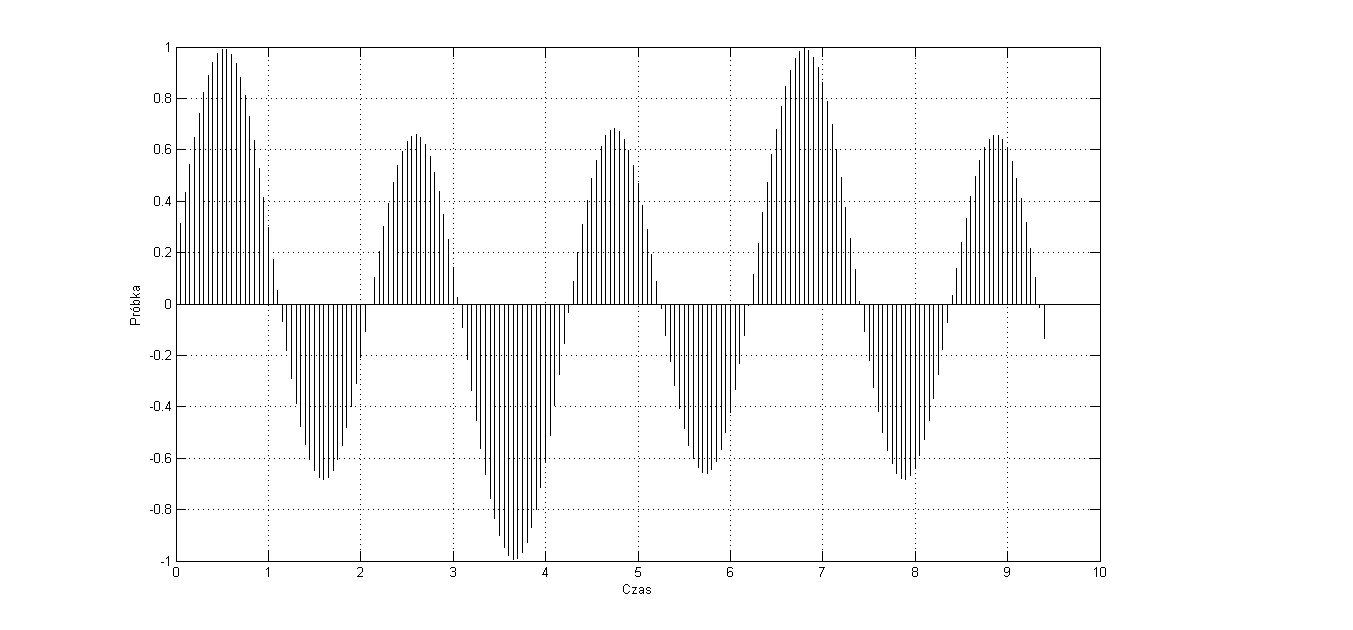
\includegraphics[width=\textwidth,trim= 3cm 0cm 6cm 0cm, clip]{./img/mfcc_wave}
			\caption{Reprezentacja sygnału ciągłego za pomocą tablicy liczb zmiennoprzecinkowych.
			Kolejne elementy tablicy zawierają wartości kolejnych próbek sygnału, i tak element o
			indeksie 0 zawiera wartość 0.0, element o indeksie 1 wartość 0.31,
			element o indeksie 2 wartość 0.43 itd.}
			\label{fig:sndwave}
		\end{figure}
		Konwersji plików WAVE na wyżej opisany format dokonaliśmy za pomocą darmowej biblioteki
		NAudio.
		
		\subsubsection*{Normowanie Sygnału Wejściowego}
		Okazuje się że w zależność od mówcy (a także jego nastroju, czy zmęczenia), oddalenia od mikrofonu
		oraz innych czynników można otrzymać dość znaczne różnice w amplitudzie nagrywanych sygnałów
		dźwiękowych. Aby wyeliminować wpływ amplitudy sygnału na jakość klasyfikacji wszystkie przetwarzane
		sygnały przed ekstrakcją cech są poddawane normowaniu. 
		Algorytm normujący sygnał wejściowy został przedstawiony
		na listingu \ref{alg:normsignal}. 
		\begin{algorithm}[h]
			\begin{algorithmic}[1]
				\STATE \COMMENT{$samples_i$ - Array containing voice samples}
				\STATE empth $\leftarrow$ 1.0
				\STATE max $\leftarrow max_i(samples_i)$
				\STATE min $\leftarrow min_i(samples_i)$
				\STATE
				\IF{$|min| > \epsilon$}
					\STATE emph $\leftarrow$ $\max(emph, \frac{1}{|min|})$
				\ENDIF
				\IF{$|max| > \epsilon$}
					\STATE emph $\leftarrow \min(emph, \frac{1}{|max|});$
				\ENDIF
				\STATE
				\FORALL{i}
					\STATE $samples_i \leftarrow emph \cdot samples_i$
				\ENDFOR
			\end{algorithmic}			
			\caption{Algorytm wykorzystywany do unormowania wartości sygnału wejściowego}
			\label{alg:normsignal}
		\end{algorithm}
		
		\subsubsection*{Algorytm Ekstrakcji Cech}
		W tej części dokumentu przedstawimy algorytmy służące do 
		wyodrębniania charakterystycznych cech mowy, omówimy również
		towarzyszące im parametry. Tabela \ref{tab:ftextractparams} zawiera
		opis parametrów algorytmów, listingi \ref{alg:ftextract}, \ref{alg:extractframe}
		oraz \ref{alg:getmfcc} prezentują pseudokody wykorzystywanych algorytmów.
		\begin{table}[h]
			\centering
			\begin{tabular}{|p{2.5cm}|c|p{6cm}|}
				\hline
				Parametr & Optymalna wartość & Opis parametru \\
				\hline \hline
				WINDOW-SIZE & 512 - 1024 & Określa ile próbek tworzy pojedynczą
				ramkę. Wielkość okna powinna być tak dobrana żeby czas trwania ramki
				wynosił od 10 do 30 milisekund. Wartość tego parametru powinna być potęgą liczby 2\\
				\hline
				WINDOW-OVERLAP & 256 - 512 & Określa ile próbek współdzielą ze sobą sąsiadujące ramki\\
				\hline
				SPEAK\-POWER\-THRESHOLD & 0.02 - 0.06 & Parametr określa minimalną energie jaką musi
				posiadać sygnał dźwiękowy żeby został uznany za część wypowiedzi \\
				\hline
				MFCC-COUNT & 6 - 16 & Ilość używanych współczynników MFCC \\				
				\hline
				$|\bigtriangleup|$ & 24 - 27 & Ilość używanych filtrów trójkątnych. Filtry pokrywają
				pasmo częstotliwości od 0~Hz do 8~kHz zgodnie ze skalą MEL. Aby utworzyć zbiór filtrów
				wymagana jest znajomość częstotliwości próbkowania $F$, oraz rozmiar ramki WINDOW-SIZE. 
				Rysunek \ref{fig:trifilter} przedstawia przepustowość oraz rozmieszczenie
				przykładowego zestawu filtrów \\
				\hline				
				$\bigtriangleup_i^n$ & & Przepustowość filtra o numerze $n$ dla częstotliwości odpowiadającej
				$i$-temu wyjściu transformacji Furiera \\
				\hline
			\end{tabular}			
			\caption{Opis parametrów algorytmu ekstrakcji cech}
			\label{tab:ftextractparams}
		\end{table}
		\begin{figure}[h]
			\includegraphics[width=\textwidth,trim= 0cm 0cm 0cm 0cm, clip]{./img/triFilter}
			\caption{Położenie i przepustowość banku filtrów trójkątnych rozłożonych zgodnie 
			ze skalą MEL na przedziale częstotliwości 0Hz - 8kHz}
			\label{fig:trifilter}
		\end{figure}
		
		\begin{algorithm}[h]
			\begin{algorithmic}[1]
				\STATE \textbf{input} samples $:$ \textbf{array} $[0 .. (N-1)]$ \textbf{of double}
				\STATE
				\STATE \COMMENT{Type \textbf{mfcc} is used to represent array of MFCC coefficients}
				\STATE \textbf{type mfcc} $=$ \textbf{array} $[0 .. ($MFCC-COUNT$-1)]$ \textbf{of double}
				\STATE features	$:$ \textbf{list} \textbf{of mfcc}			
				\STATE start $\leftarrow 0$
				\STATE delta $\leftarrow$ WINDOW-SIZE $-$ WINDOW-OVERLAP
				\STATE
				\WHILE{start $<$ N - WINDOW-SIZE}
					\STATE frame $\leftarrow$ ExtractFrame(samples, start)
					\STATE power $\leftarrow \sum_i |frame_i| /$ WINDOW-SIZE
					\IF{power $>$ SPEAK-POWER-THRESHOLD}
						\STATE mfcc $\leftarrow$ GetMFCC(frame)
						\STATE \textbf{append} mfcc \textbf{to} features
					\ENDIF					
					\STATE start $\leftarrow$ start + delta
				\ENDWHILE
				\STATE
				\RETURN features
			\end{algorithmic}			
			\caption{Algorytm wykorzystywany do ekstrakcji cech z sygnału wejściowego}
			\label{alg:ftextract}
		\end{algorithm}	
		\begin{algorithm}[h]
			\begin{algorithmic}[1]
				\STATE \textbf{input} samples $:$ \textbf{array} $[0 .. (N-1)]$ \textbf{of double}
				\STATE \textbf{input} start $:$ \textbf{integer}
				\STATE
				\STATE frame $:$ \textbf{array} $[0 .. ($WINDOW-SIZE$-1)]$ \textbf{of double}
				\FOR{$0 \leq i < $ WINDOW-SIZE}
					\STATE $frame_i$ = $samples_{start+i}$
				\ENDFOR
				\STATE
				\RETURN frame
			\end{algorithmic}			
			\caption{ExtractFrame - Procedura pomocnicza}
			\label{alg:extractframe}
		\end{algorithm}	
		\begin{algorithm}[h]
			\begin{algorithmic}[1]
				\STATE \textbf{input} frame $:$ \textbf{array} $[0 .. (N-1)]$ \textbf{of double}
				\STATE
				\FOR{$0 \leq i < N$}
					\STATE $hamming_i \leftarrow 0.54 - 0.46 \cos(\frac{2\pi i}{N - 1})$
					\STATE $frame_i \leftarrow hamming_i \cdot frame_i$
				\ENDFOR
				\STATE
				\STATE $furier \leftarrow$ \textbf{FFT} $(frame)$
				\FOR{$0 \leq i < N$}
					\STATE $furier_i \leftarrow |furier_i|$
				\ENDFOR
				\STATE
				\FOR{$0 \leq i < |\bigtriangleup|$}
					\STATE $sum_i \leftarrow 0$
					\FOR{$0 \leq j < N$}
						\STATE $sum_i \leftarrow sum_i + \bigtriangleup_j^i \cdot furier_j$					
					\ENDFOR
					\STATE $sum_i \leftarrow \log_{10}(sum_i)$
				\ENDFOR
				\STATE
				\STATE \COMMENT{Return only first MFCC-COUNT elements of array returned by DCT}
				\RETURN \textbf{DCT}(sum)
			\end{algorithmic}			
			\caption{GetMFCC - Algorytm obliczania współczynników MFCC dla danej ramki}
			\label{alg:getmfcc}
		\end{algorithm}	

	\clearpage
	\subsection{Opis Algorytmu Rozpoznawania Mówcy}
	
		Listing \ref{alg:recognise} zawiera pseudokod algorytmu wykorzystywanego 
		do wytypowania najbardziej prawdopodobnego mówcy, tabela \ref{tab:srparams}
		zawiera opis parametrów występujących w algorytmie.
		\begin{table}[h]
			\centering
			\begin{tabular}{|c|c|p{6cm}|}
				\hline
				Parametr & Optymalna wartość & Opis parametru \\
				\hline \hline
				$T$ & 0.65 $\pm$ 0.05 & Próg wiarygodności sieci neuronowej. Odpowiedz sieci będzie
				uznana za znaczącą wtedy gdy będzie należeć do sumy przedziałów $[0, 1-T]$ oraz
				$[T, 1]$ \\
				\hline
				Features &  & Tablica współczynników MFCC dla ramek rozpoznawanego sygnału mowy \\
				\hline
				People & & Zbiór osób rozpoznawanych przez klasyfikator \\
				\hline
				$network_{person}$ & & Sieć neuronowa nauczona rozpoznawania osoby $person$ oraz 
				odrzucania pozostałych osób \\
				\hline
				FRAMES-COUNT & 6 - 16 & Parametr określający ile kolejnych ramek 
				(a raczej odpowiadających im tablic
				współczynników MFCC) jest podawanych na wejście sieci neuronowej. Wielkość wejścia sieci
				można policzyć mnożąc FRAMES-COUNT przez MFCC-COUNT \\
				\hline
			\end{tabular}			
			\caption{Opis parametrów algorytmu wyboru zwycięzcy}
			\label{tab:srparams}
		\end{table}		
		\begin{algorithm}
			\begin{algorithmic}[1]
				\STATE \textbf{input} Features $:$ \textbf{array} $[0 .. (N-1)]$ \textbf{of mfcc}
				\STATE				
				\STATE total $\leftarrow$ 0
				\FORALL{person $\in$ People}
					\STATE $result_{person}$ $\leftarrow$ 0
				\ENDFOR
				\STATE
				\FORALL{0 $\leq$ start $<$ N - FRAMES-COUNT}
					\STATE \COMMENT{Skopiuj elementy tablicy features do tablicy netinput}
					\STATE \COMMENT{Kopiujemy również oba indeksy graniczne}
					\STATE netinput $\leftarrow$ Features$[$start$ .. ($start $+$ FRAMES-COUNT$-1)]$
					\STATE
					\FORALL{person $\in$ People}
						\STATE answer = $network_{person}($netinput$)$
						\IF{answer $>$ T \textbf{or} answer $<$ (1 - T)}
							\IF{answer $>$ T}
								\STATE $result_{person}$ $\leftarrow$ $result_{person}$ $+$ answer
								\STATE total $\leftarrow$ total + 1
							\ELSE
								\STATE $result_{person}$ $\leftarrow$ $result_{person}$ $+$ (answer - 1)
							\ENDIF
							\STATE \COMMENT{Notice that total is incremented only in the first branch}
						\ENDIF	
					\ENDFOR
				\ENDFOR
				\STATE
				\FORALL{person $\in$ People}
					\STATE $result_{person}$ $\leftarrow$ $max(0, result_{person} / total)$
				\ENDFOR
				\STATE \textbf{sort descend} person \textbf{by} $result_{person}$
			\end{algorithmic}			
			\caption{RecogniseSpeaker - Algorytm rozpoznawania mówcy}
			\label{alg:recognise}
		\end{algorithm}
		\clearpage
	
\section{Omówienie Uzyskanych Wyników}
	\subsection{Metodologia testowania}
	
	Dla wszystkich przedstawionych w dalszej części dokumentu testów jako 
	konfigurację bazową przyjmiemy następujące wartości parametrów sieci neuronowej:
	\begin{table}[h]
			\centering
			\begin{tabular}{|c|p{8cm}|}
				\hline
				Parametr &  Wartość \\
				\hline \hline
				$D_1$, $D_2$ & Parametry te mają odpowiednio wartości 4 i 8 \\
				\hline
				MAX-ERROR & Wartość 0.0 \\
				\hline
				T & Wartość 0.65 \\
				\hline
				WINDOW-SIZE & Wartość 512 \\
				\hline
				OVERLAP & Wartość 256 \\
				\hline
				TCOEF & Wartość 0.5 \\
				\hline
				MAX-ITERATIONS & Wartość 160 tysięcy \\
				\hline
				$\eta$, $\mu$ & 0.2109, 0.105 \\
				\hline
				FRAMES-COUNT & 6 \\
				\hline
				MFCC-COUNT & 12 \\
				\hline
				$|\bigtriangleup|$ & 24 (Ilość filtrów) \\
				\hline
			\end{tabular}			
			\caption{Bazowa konfiguracja testowa programu}
			\label{tab:testparams}
		\end{table}	
			
	\subsection{Wpływ Parametrów na Rezultaty}
		\subsubsection*{Zależność błędu od ilości uczonych osób}	
			\begin{figure}[h]
				\centering
				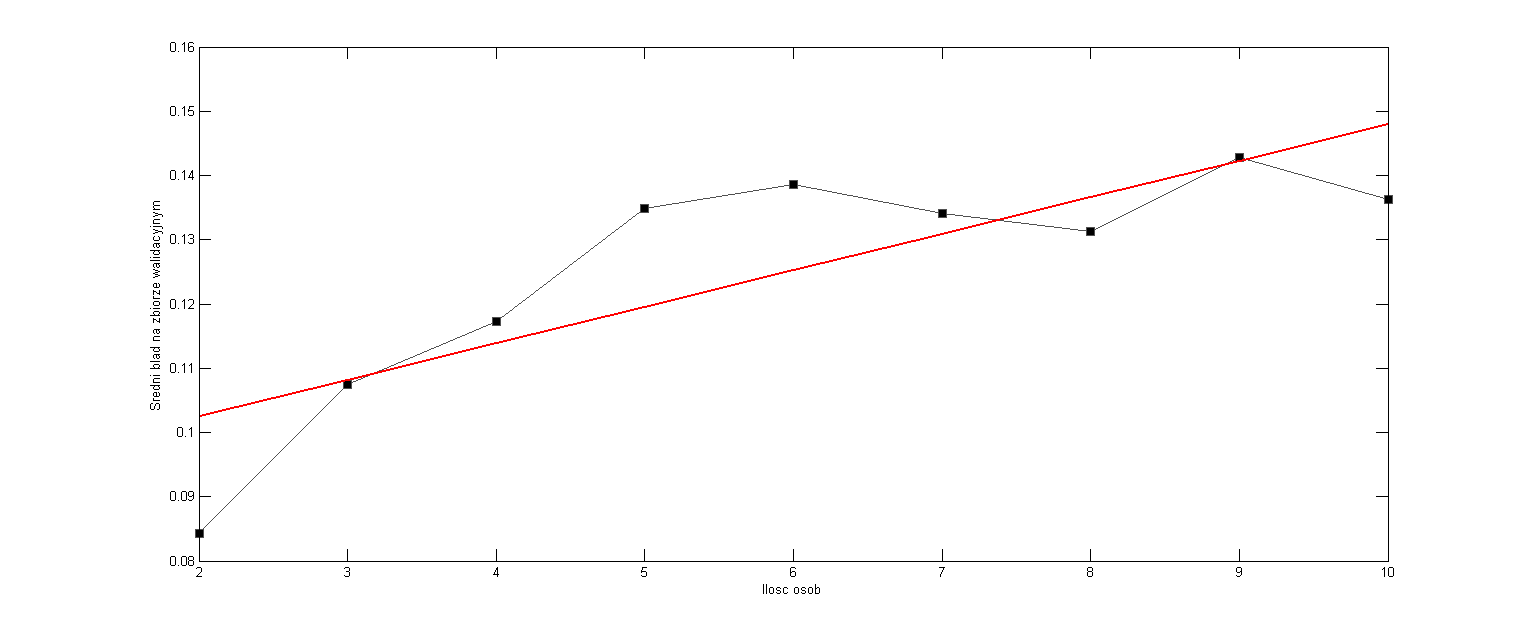
\includegraphics[width=\textwidth,trim= 3cm 0cm 3cm 0cm, clip]{./img/b_od_lo}
				\caption{Średni błąd sieci na zbiorze walidacyjnym w zależności od liczby uczonych osób.
				Na \textcolor{red}{czerwono} wykreślono linie regresji. Zauważmy że w przyjętej metodologii
				liczenia błędu, błąd rzędu 0.16 powoduje że odpowiedzi sieci różnią się od oczekiwanych
				o około $\sqrt{0.16} = 0.4$ co praktycznie uniemożliwia działanie aplikacji przy T równym
				0.65. Z kolei zbyt wysoka wartość T może spowodować że wyniki będą w dużej mierze losowe.}
				\label{fig:bodilos}
			\end{figure}
			\begin{figure}[h]
				\centering
				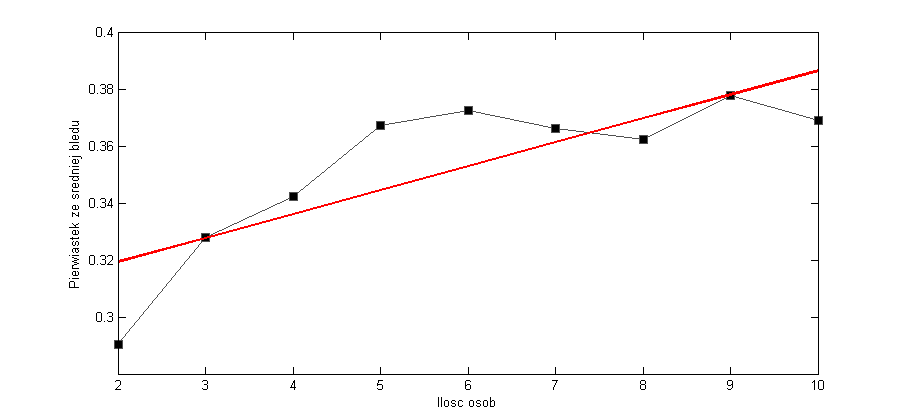
\includegraphics[width=\textwidth,trim= 1cm 0cm 1cm 0cm, clip]{./img/b_od_lo2}
				\caption{Pierwiastek błędu sieci na zbiorze walidacyjnym w zależności od liczby uczonych osób.
				Na \textcolor{red}{czerwono} wykreślono linie regresji. Błąd rzędu $0.35$ przy T równym
				$0.65$ jest akceptowalny.}
				\label{fig:bodilosd}
			\end{figure}
			Wzrost liczby osób rozpoznawanych przez sieć powoduje wzrost błędu
			zespołu sieci neuronowych. Możemy przyjąć że rozpoznawanie powyżej sześciu osób obarczone jest
			znacznych błędem, przy T równym 0.65.
			
	\subsection{Przebieg nauki zespołu sieci neuronowych}
		Wykres \ref{fig:ttresults} przedstawiony w tej części dokumentu 
		prezentuje błąd sieci w zależności od liczby iteracji
		algorytmu backpropagation. Widzimy że w niektórych przypadkach nauka sieci jest 
		praktycznie niemożliwa co jest spowodowane złą jakością zebranych próbek (np. różny
		charakter głosu danej osoby w każdej próbce). Dodatkowo w przypadku niektórych osób widać
		wyraźny rozdźwięk pomiędzy błędem na zbiorze uczącym i walidacyjnym, oznacza to że
		zbiór walidacyjny zawiera istotne cechy głosu danej osoby nieobecne w zbiorze uczącym.
		Wynika z stąd że próbki uczące powinny być jak najdłuższe oraz jak najbardziej różnorodne (tj. zawierać
		jak najwięcej różnych sylab),
		przy zachowaniu tej samej barwy oraz tempa wypowiedzi - co niestety nie jest zbyt praktycznym założeniem.
	\subsection{Jakość rozpoznawania w zależności od odległości mówcy od mikrofonu}
		Z doświadczeń płynących z pracy z aplikacją wynika że zmniejszenie odległości od mikrofonu 
		pozytywnie wpływa na jakość rozpoznawania. Okazuje się jednak że odległość (w ograniczonym zakresie
		wartości) nie ma aż tak dużego znaczenia dla odpowiedzi sieci neuronowej. Wykresy
		\ref{fig:netansblisko} oraz \ref{fig:netansdaleko} przedstawiają odpowiedzi sieci dla dwóch badanych
		odległości (szczegóły w opisach rysunków). W przypadku I aplikacją była trochę bardziej pewna rozpoznawanej
		osoby (25\% w stosunku do 20\% w drugim przypadku).
	 
		\clearpage
		\newpage	
		\thispagestyle{empty}
		\addtolength{\voffset}{-105pt}
	
		\begin{figure}[h]	
  		\centering
\subfloat[Adrian Sroka]{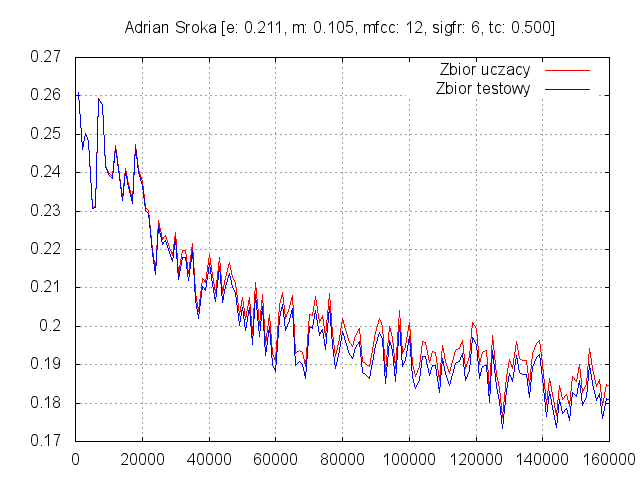
\includegraphics[scale=0.25]{./img/plot_Adrian_Sroka.png}}
\subfloat[Albert Skłodowski]{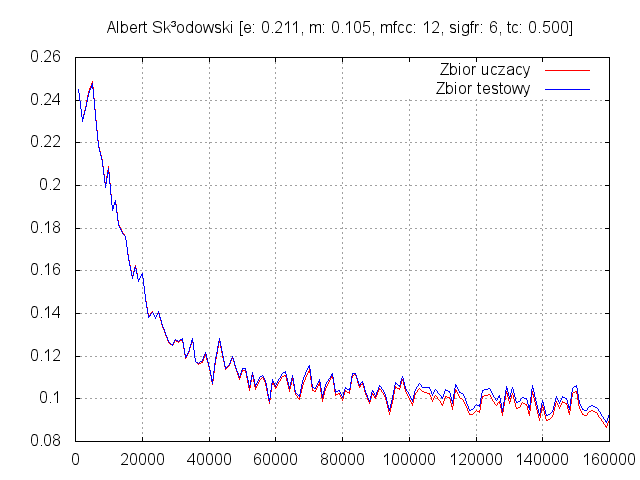
\includegraphics[scale=0.25]{./img/plot_Albert_Sklodowski.png}}\\
\subfloat[Andrzej Legucki]{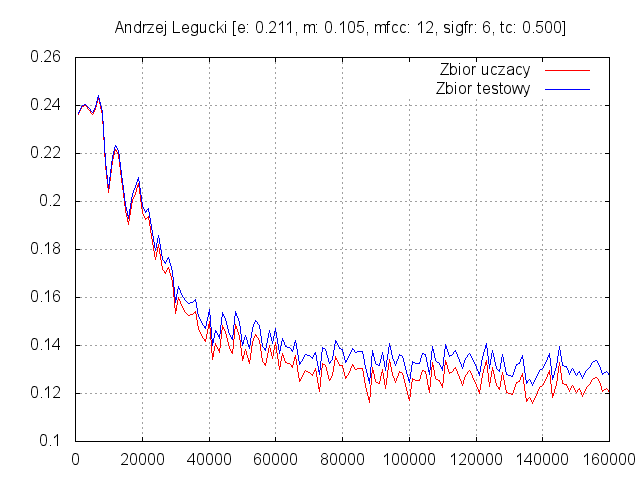
\includegraphics[scale=0.25]{./img/plot_Andrzej_Legucki.png}}
\subfloat[Artur Adamek]{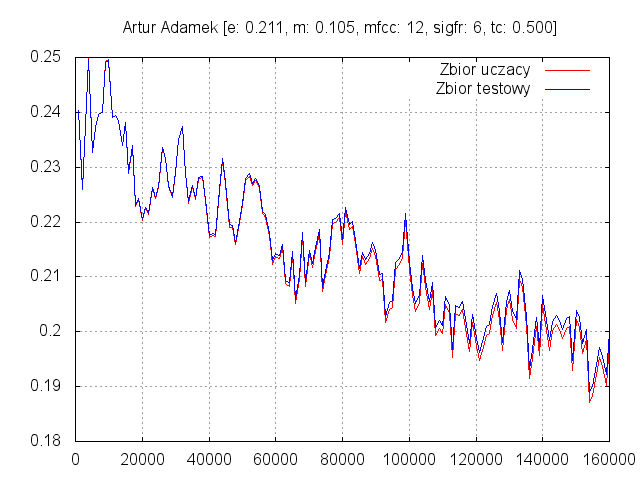
\includegraphics[scale=0.25]{./img/plot_Artur_Adamek.png}}\\
\subfloat[Janusz Paprzycki]{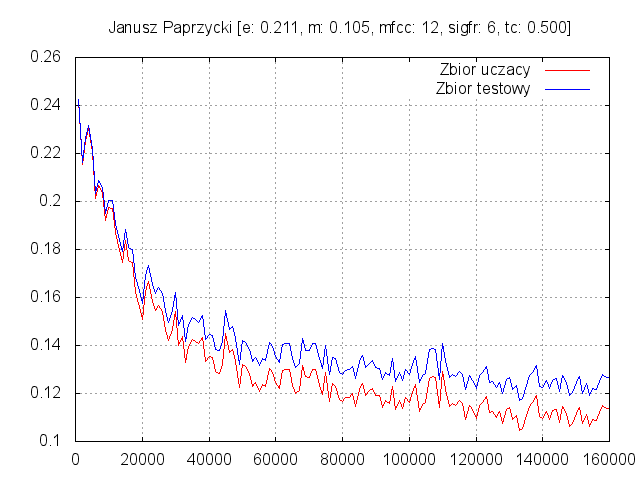
\includegraphics[scale=0.25]{./img/plot_Janusz_Paprzycki.png}}
\subfloat[Julian Zubek]{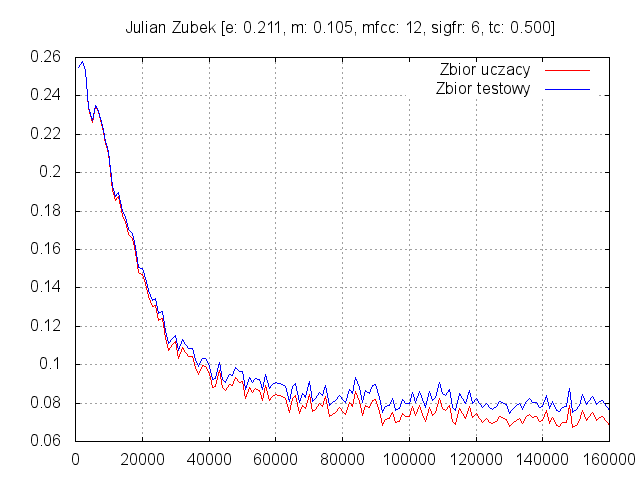
\includegraphics[scale=0.25]{./img/plot_Julian_Zubek.png}}\\
\subfloat[Mai Hoa Pham]{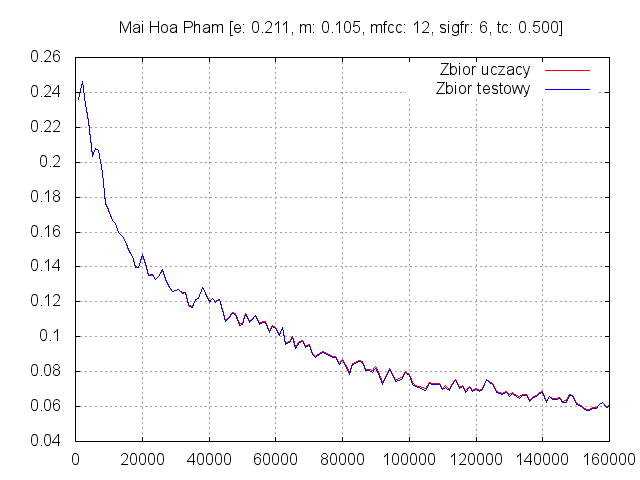
\includegraphics[scale=0.25]{./img/plot_Mai_Hoa_Pham.png}}
\subfloat[Marcin Chwedczuk]{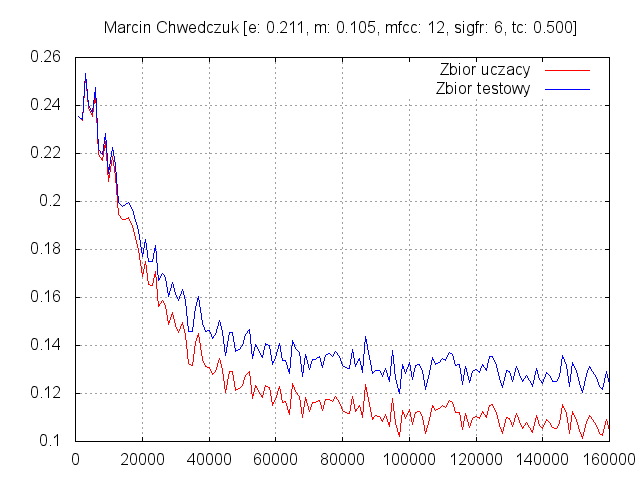
\includegraphics[scale=0.25]{./img/plot_Marcin_Chwedczuk.png}}\\
\subfloat[Michał Okulewicz]{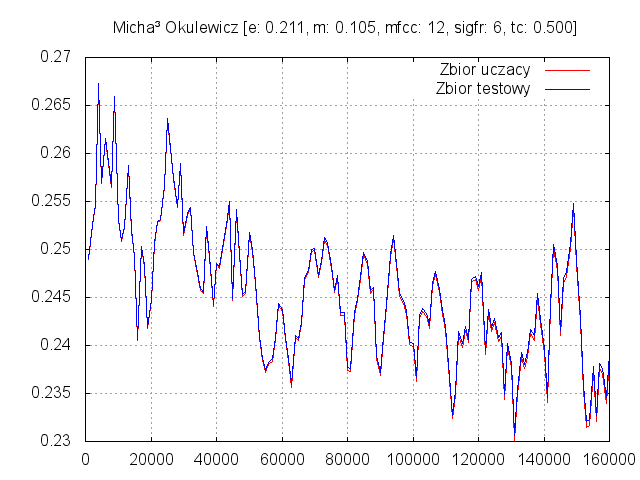
\includegraphics[scale=0.25]{./img/plot_Michal_Okulewicz.png}}
\subfloat[Tomek Sitarek]{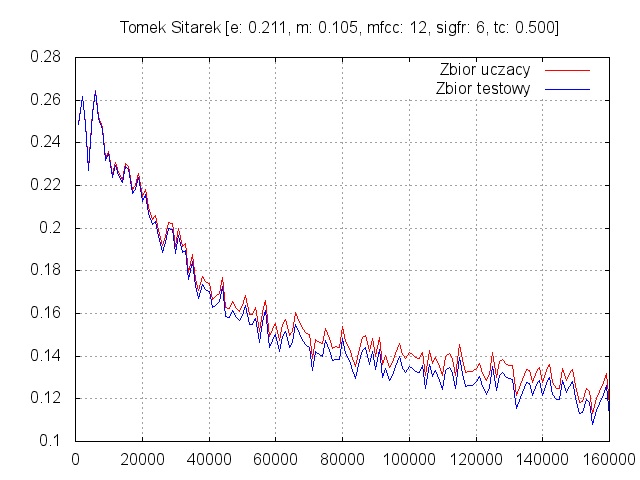
\includegraphics[scale=0.25]{./img/plot_Tomek_Sitarek.png}}
  		\caption{Wykresy przedstawiają wielkość błędu w zależności od liczby iteracji.
  		Kolorem \textcolor{blue}{niebieskim} wykreślono błąd na zbiorze walidacyjnym,
  		a kolorem \textcolor{red}{czerwonym} na zbiorze uczącym.
  		Oś Y przedstawia błąd średniokwadratowy, oś X liczbę iteracji nauki.}
  		\label{fig:ttresults}
	\end{figure}
	\clearpage
	
	\newpage	
	\thispagestyle{empty}
		\begin{figure}[h]	
  		\centering
\subfloat[Adrian Sroka]{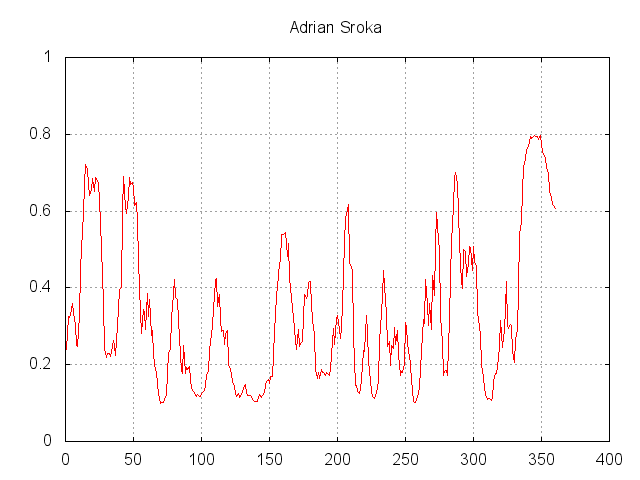
\includegraphics[scale=0.25]{./img/blisko/rplot_Adrian_Sroka.png}}
\subfloat[Albert Skłodowski]{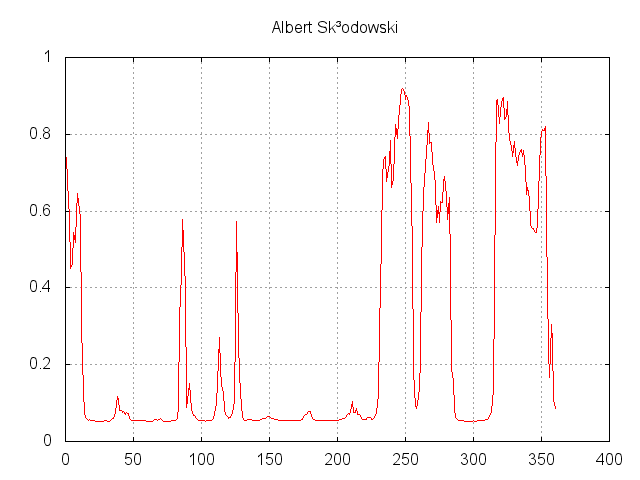
\includegraphics[scale=0.25]{./img/blisko/rplot_Albert_Sklodowski.png}}\\
\subfloat[Andrzej Legucki]{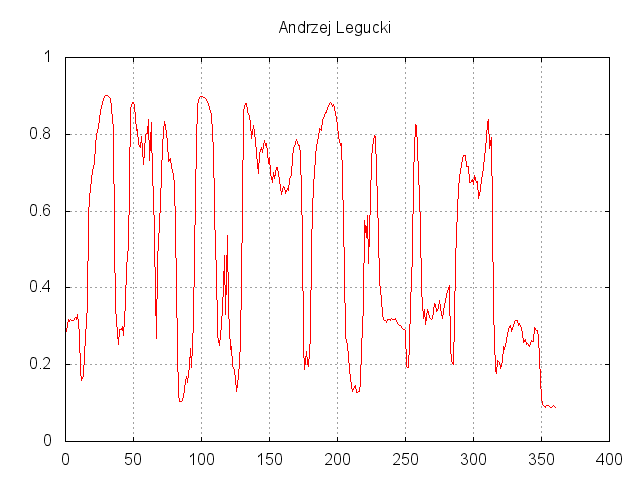
\includegraphics[scale=0.25]{./img/blisko/rplot_Andrzej_Legucki.png}}
\subfloat[Artur Adamek]{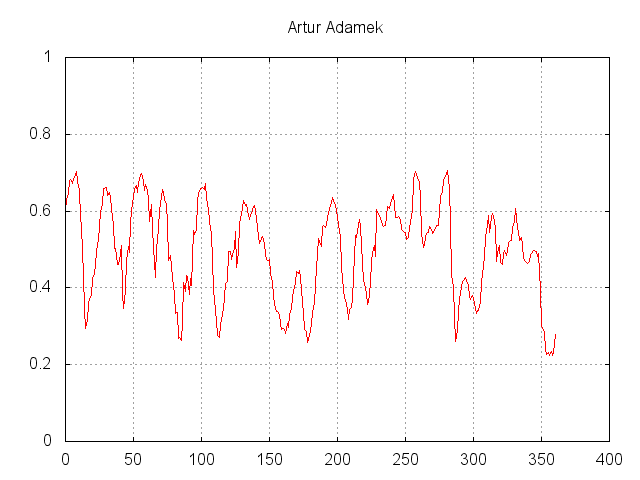
\includegraphics[scale=0.25]{./img/blisko/rplot_Artur_Adamek.png}}\\
\subfloat[Janusz Paprzycki]{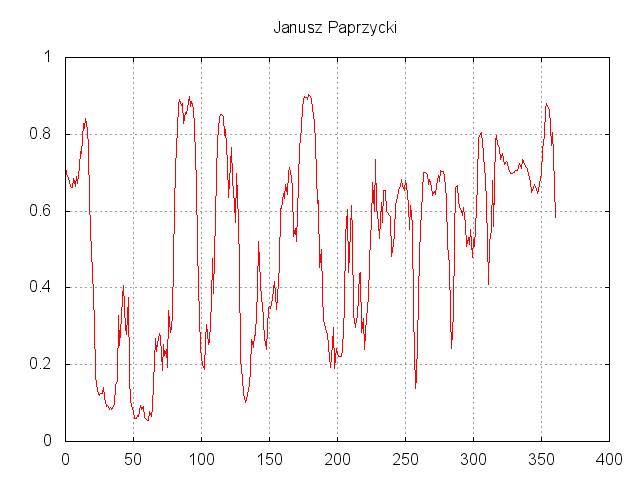
\includegraphics[scale=0.25]{./img/blisko/rplot_Janusz_Paprzycki.png}}
\subfloat[Julian Zubek]{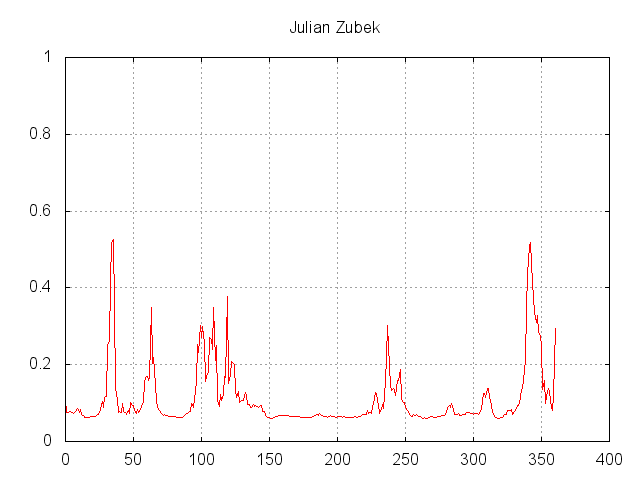
\includegraphics[scale=0.25]{./img/blisko/rplot_Julian_Zubek.png}}\\
\subfloat[Mai Hoa Pham]{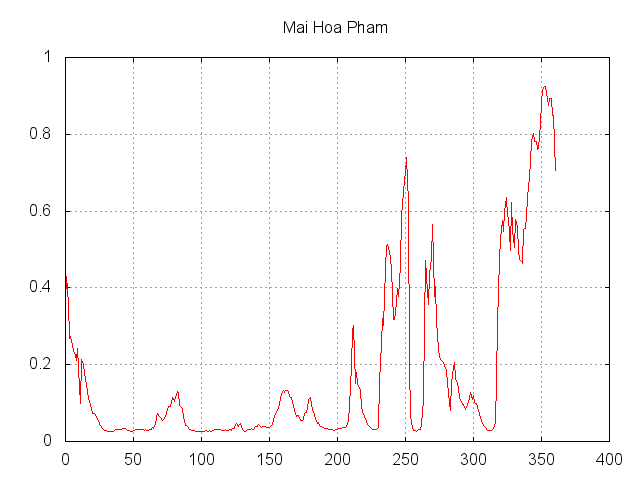
\includegraphics[scale=0.25]{./img/blisko/rplot_Mai_Hoa_Pham.png}}
\subfloat[Marcin Chwedczuk]{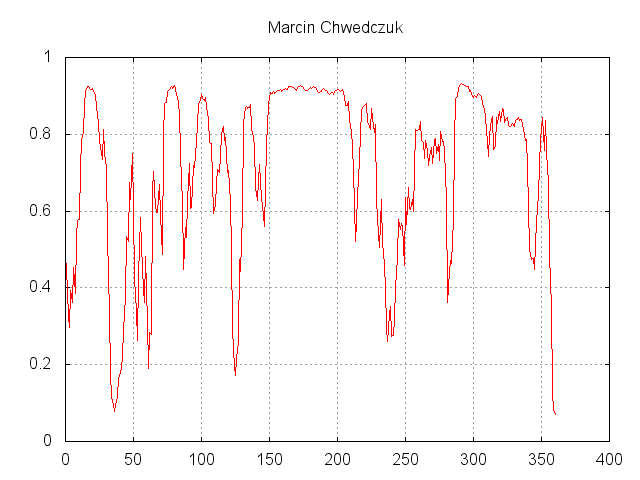
\includegraphics[scale=0.25]{./img/blisko/rplot_Marcin_Chwedczuk.png}}\\
\subfloat[Michał Okulewicz]{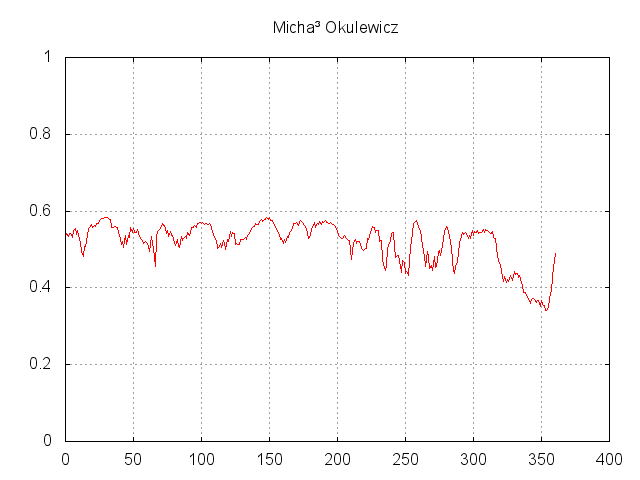
\includegraphics[scale=0.25]{./img/blisko/rplot_Michal_Okulewicz.png}}
\subfloat[Tomek Sitarek]{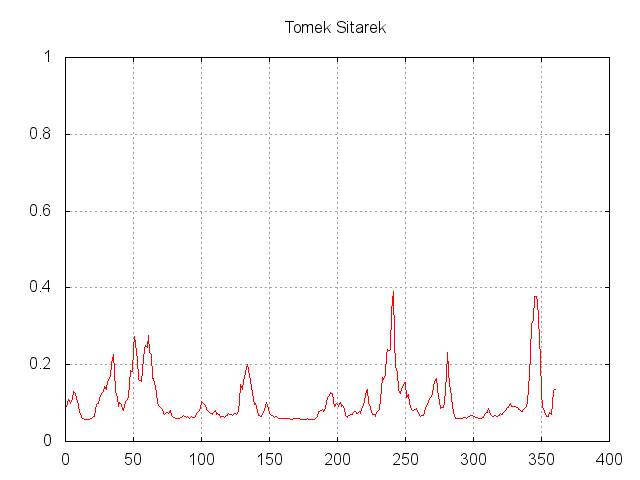
\includegraphics[scale=0.25]{./img/blisko/rplot_Tomek_Sitarek.png}}
  		\caption{Wykresy przedstawiają odpowiedzi poszczególnych sieci na 
  		frazę \textit{Twórcy Oprogramowania Przyszłości}. Fraza została nagrana przy \textbf{niewielkiej} (ok. 5cm)
  		odległości ust od mikrofonu. Oś X odpowiada początkowemu indeksowi zestawu 12 ramek MFCC. Osobą
  		mówiącą był Marcin Chwedczuk}
  		\label{fig:netansblisko}
	\end{figure}	
	
	\clearpage
	\newpage	
	\thispagestyle{empty}
		\begin{figure}[h]	
  		\centering
\subfloat[Adrian Sroka]{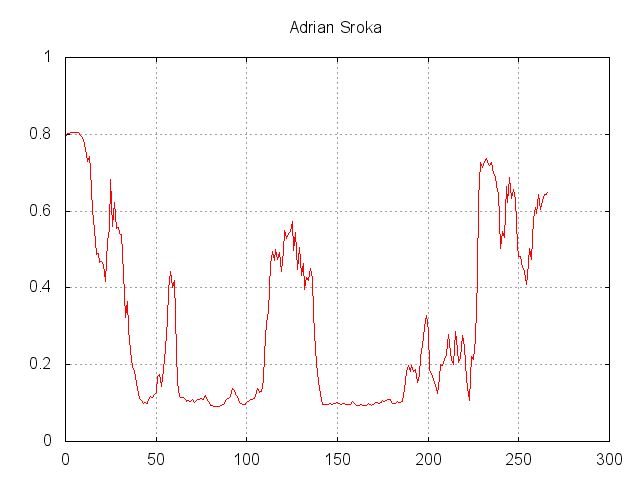
\includegraphics[scale=0.25]{./img/polmetra/rplot_Adrian_Sroka.png}}
\subfloat[Albert Skłodowski]{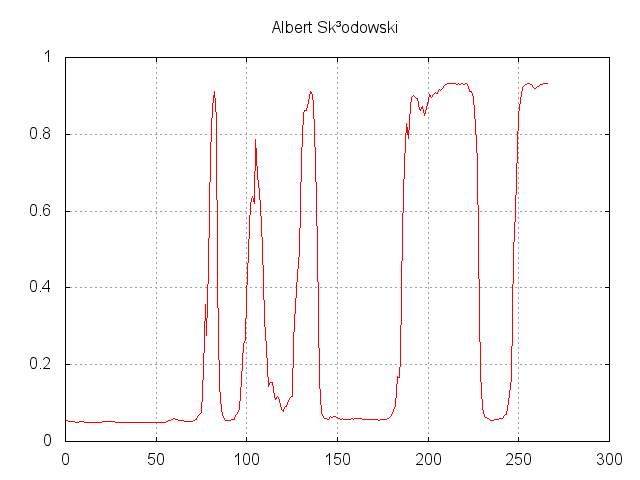
\includegraphics[scale=0.25]{./img/polmetra/rplot_Albert_Sklodowski.png}}\\
\subfloat[Andrzej Legucki]{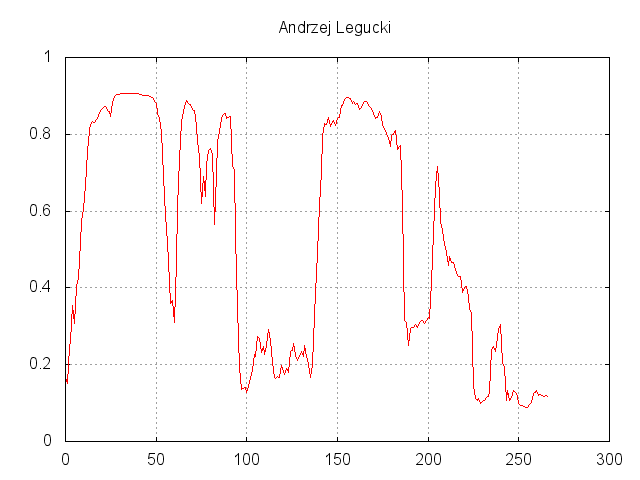
\includegraphics[scale=0.25]{./img/polmetra/rplot_Andrzej_Legucki.png}}
\subfloat[Artur Adamek]{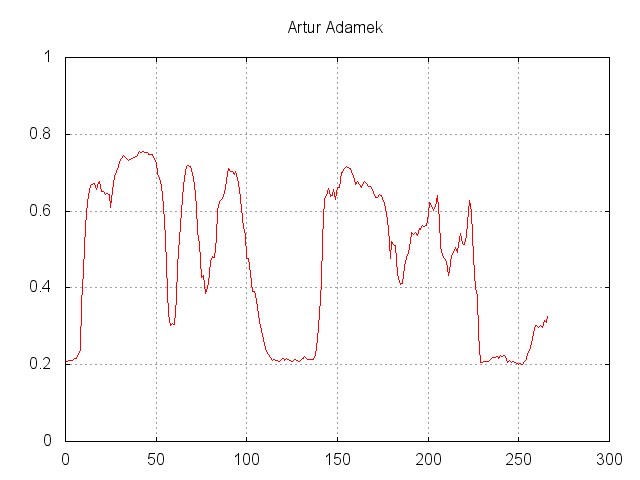
\includegraphics[scale=0.25]{./img/polmetra/rplot_Artur_Adamek.png}}\\
\subfloat[Janusz Paprzycki]{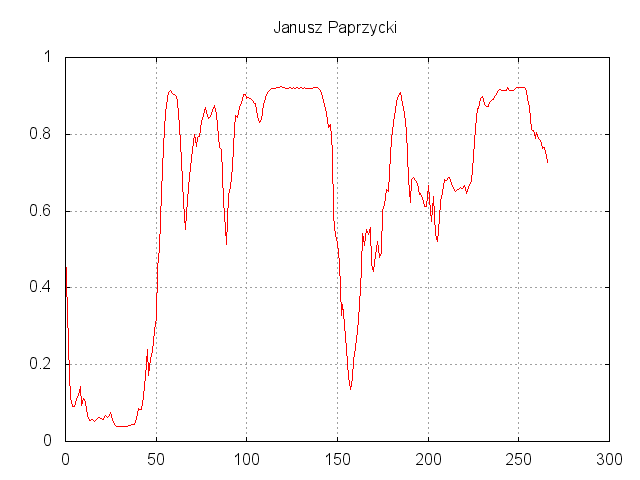
\includegraphics[scale=0.25]{./img/polmetra/rplot_Janusz_Paprzycki.png}}
\subfloat[Julian Zubek]{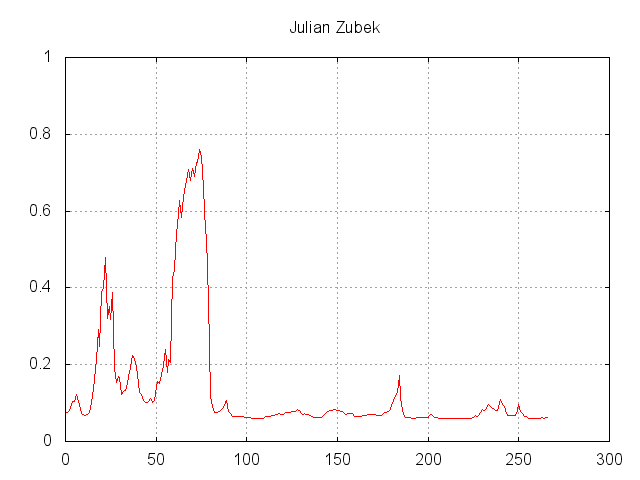
\includegraphics[scale=0.25]{./img/polmetra/rplot_Julian_Zubek.png}}\\
\subfloat[Mai Hoa Pham]{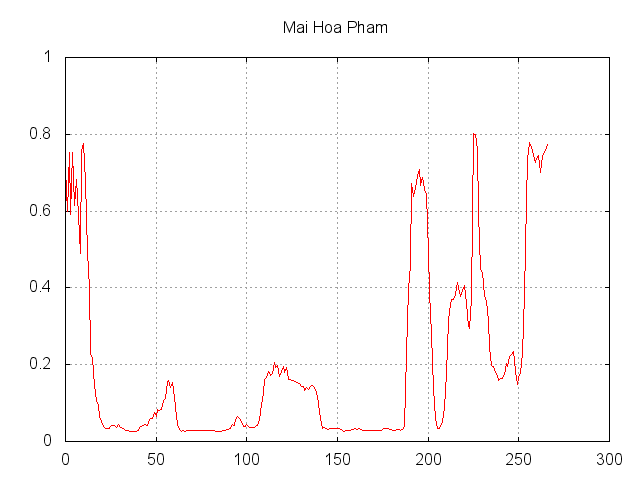
\includegraphics[scale=0.25]{./img/polmetra/rplot_Mai_Hoa_Pham.png}}
\subfloat[Marcin Chwedczuk]{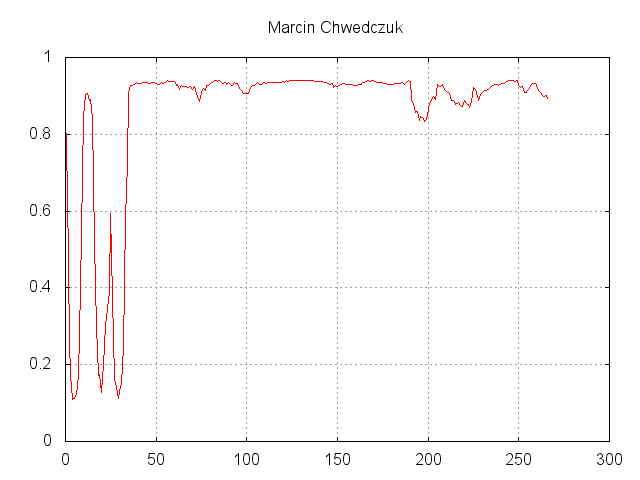
\includegraphics[scale=0.25]{./img/polmetra/rplot_Marcin_Chwedczuk.png}}\\
\subfloat[Michał Okulewicz]{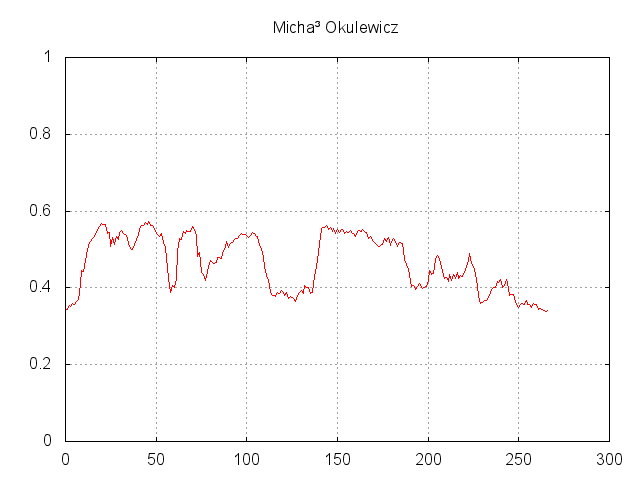
\includegraphics[scale=0.25]{./img/polmetra/rplot_Michal_Okulewicz.png}}
\subfloat[Tomek Sitarek]{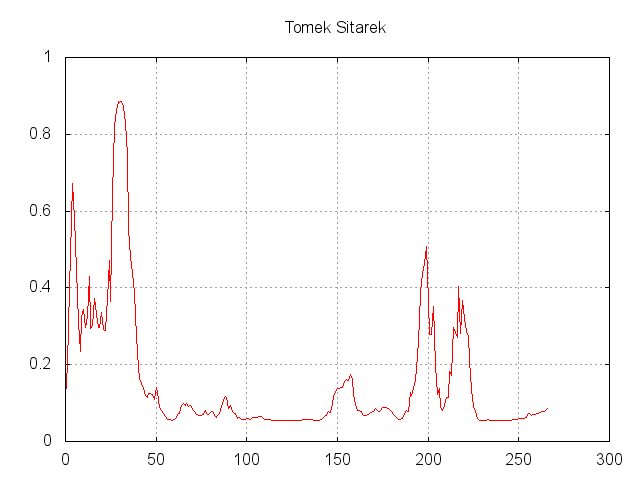
\includegraphics[scale=0.25]{./img/polmetra/rplot_Tomek_Sitarek.png}}
  		\caption{Wykresy przedstawiają odpowiedzi poszczególnych sieci na 
  		frazę \textit{Twórcy Oprogramowania Przyszłości}. Fraza została nagrana przy \textbf{dużej} (ok. 55cm)
  		odległości ust od mikrofonu. Oś X odpowiada początkowemu indeksowi zestawu 12 ramek MFCC. Osobą
  		mówiącą był Marcin Chwedczuk}
  		\label{fig:netansdaleko}
	\end{figure}	
	
	\clearpage
	\newpage
	\addtolength{\voffset}{105pt}
	\subsection{Średni błąd na zbiorze walidacyjnym w zależności od parametru T}
		Przy testowani parametru T aplikacja będzie uczona rozpoznawania pięciu osób.
		Przypomnijmy że dla T = 0.5 żadne odpowiedzi sieci nie są odrzucane.
		\begin{figure}[h]	
  		\centering
\subfloat[Błąd aplikacji]{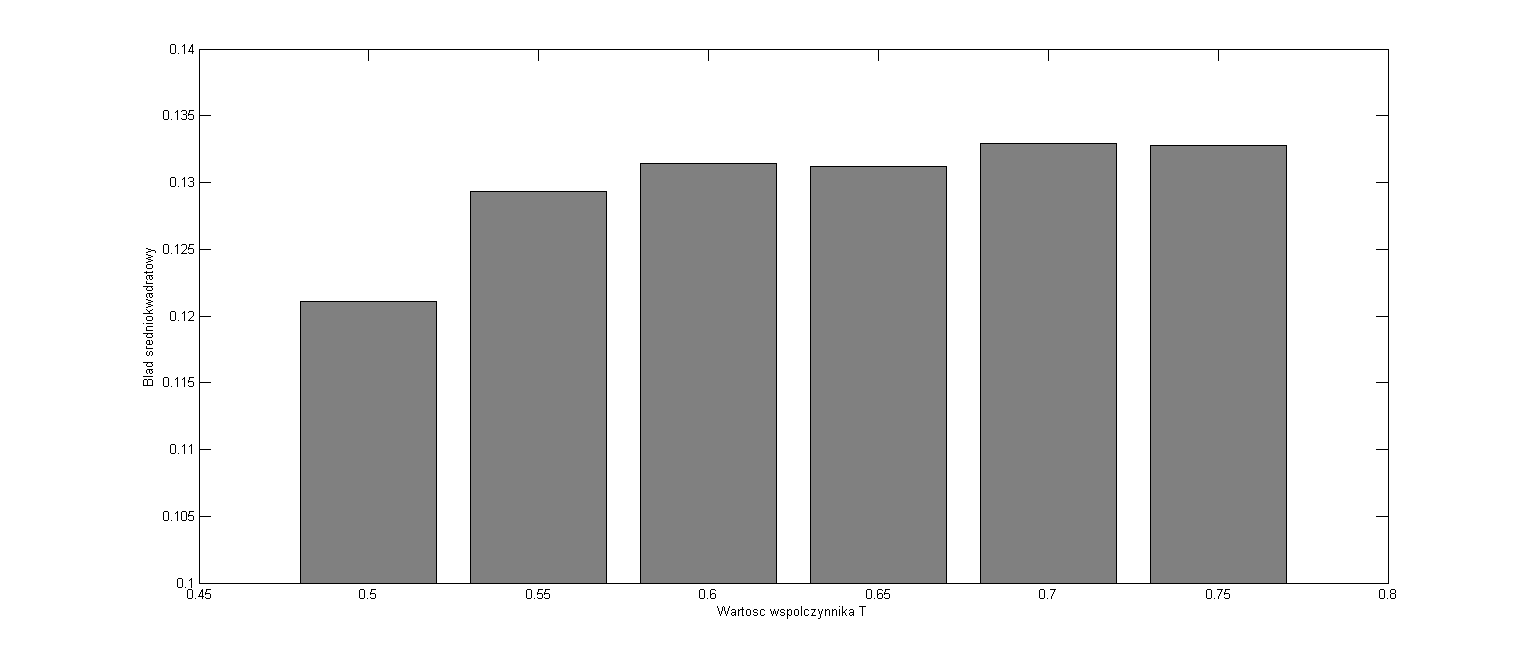
\includegraphics[width=\textwidth,trim= 3cm 0cm 3cm 0cm, clip]{./img/Tnorm}}\\
\subfloat[Pierwiastek z błędu aplikacji]{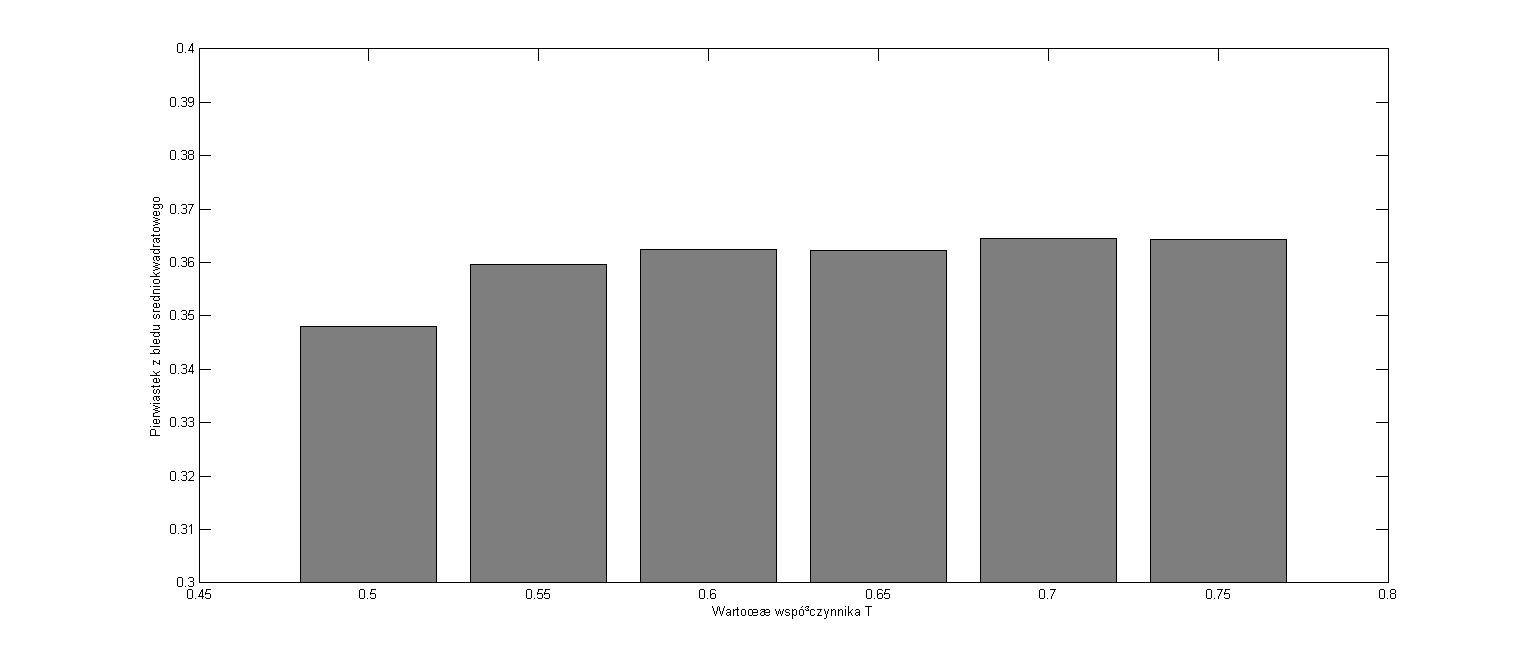
\includegraphics[width=\textwidth,trim= 3cm 0cm 3cm 0cm, clip]{./img/Tnorm2}}
  		\caption{Wykresy przedstawiają średni błąd aplikacji oraz pierwiastek z tego błędu w
  		zależności od wartości parametru T}
  		\label{fig:texp1}
	\end{figure}
	Całkiem nieoczekiwanie okazało się że ustawienie T = 0.5 nieznacznie zmniejsza błąd 
	sieci na zbiorze walidacyjnym. Podejrzewamy jednak że nie przełoży się to na skuteczność klasyfikacji,
	gdyż z naszego doświadczenia z pracy z aplikacją oraz śledzenia wykresów, wynika że wartość T nie
	powinna być ustalana poniżej 0.6. Wygląda na to że parametr T wymaga dalszych badań, 
	w rzeczywistym środowisku testowym (sala w której odbywają się zajęcia).
		
	\subsection{Średni błąd na zbiorze walidacyjnym w zależności wielkości sieci neuronowej}
		Poniższa tabela zawiera zestawienie wielkości błędu oraz parametrów $D_1$, $D_2$ 
		sterujących architekturą sieci. Sieć była uczona rozpoznawania pięciu osób.
		Z poniższych danych można wyprowadzić konkluzje że błąd na zbiorze walidacyjnym 
		maleje wraz z wzrostem rozmiaru sieci (mniejsze $D$), dzieje się to kosztem 
		wydłużonego czasu nauki (nawet rzędu 60 minut!).
		\begin{table}[h]
			\centering
			\begin{tabular}{|c|c|p{6cm}|}
				\hline
				$D_1$ & $D_2$ & Wielkość błędu \\
				\hline \hline
				\hline
					2 & 2 & 0.1226 \\
				\hline
					2 & 4 & 0.1224 \\
				\hline
					4 	& 4 & 0.1308 \\
				\hline
					3 & 5 & 0.1297 \\
				\hline
					4 & 8 & 0.1329 \\
				\hline
					8 & 16 & 0.14967 \\
				\hline
			\end{tabular}			
			\caption{Błąd w zależności od architektury sieci}
			\label{tab:srparams}
		\end{table}
		
	\subsection{Błąd na zbiorze walidacyjnym w zależności od FRAMES-COUNT}
	\begin{figure}[h]	
  		\centering
		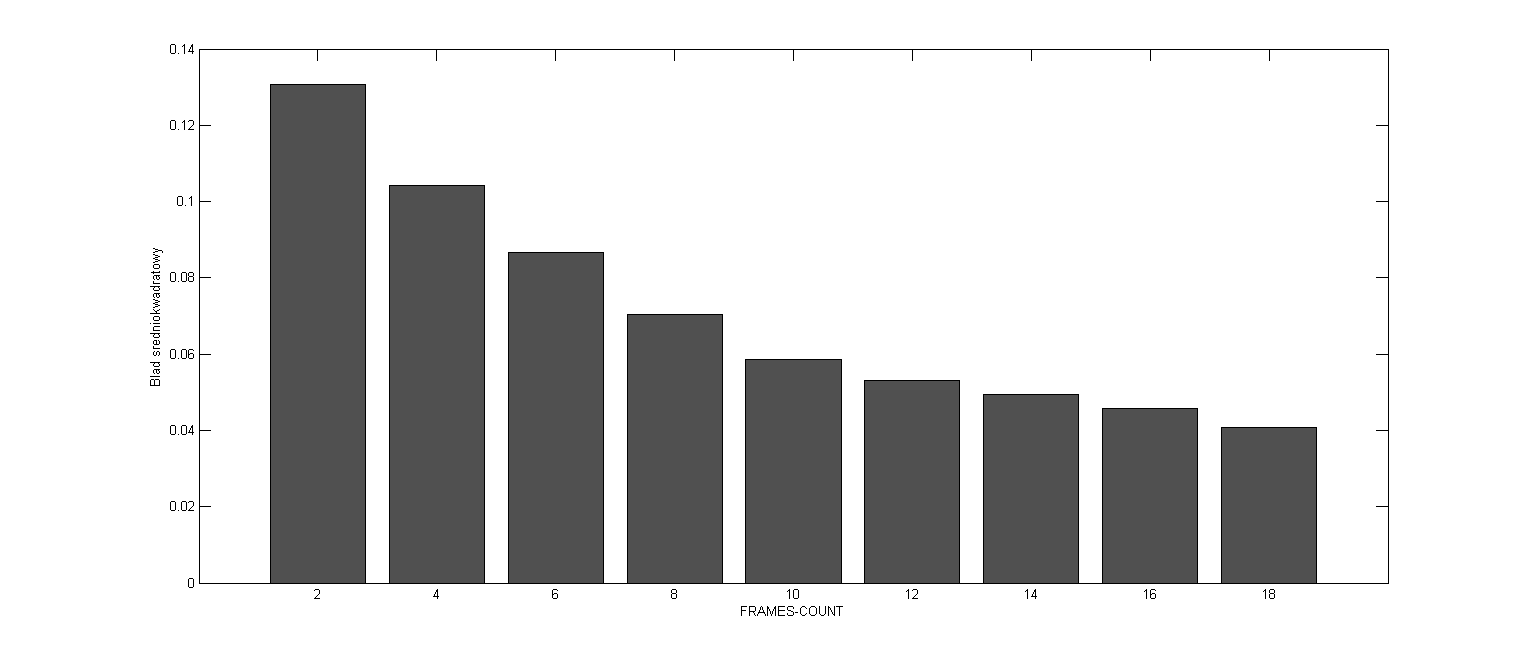
\includegraphics[width=\textwidth,trim= 3cm 0cm 3cm 0cm, clip]{./img/mfcc}
  		\caption{Wykres prezentuje zależność błędu na zbiorze walidacyjnym od współczynnika
  		FRAMES-COUNT}
  		\label{fig:mfcc1}
	\end{figure}
	Na rysunku \ref{fig:mfcc1} przedstawiono zależność błędu na zbiorze walidacyjnym od wartości 
	współczynnika FRAMES-COUNT. Z wykresu wynika że wraz z wzrostem parametru błąd ulega zmniejszeniu.
	Wydaje się że optymalna wartość tego parametru wynosi 12 (dalszy wzrost powoduje jedynie niewielką
	poprawę błędu w stosunku do zwiększonego czasu potrzebnego na naukę sieci).
		
	\subsection{Błąd na zbiorze walidacyjnym w zależności od MFCC-COUNT}
	\begin{figure}[h]	
  		\centering
		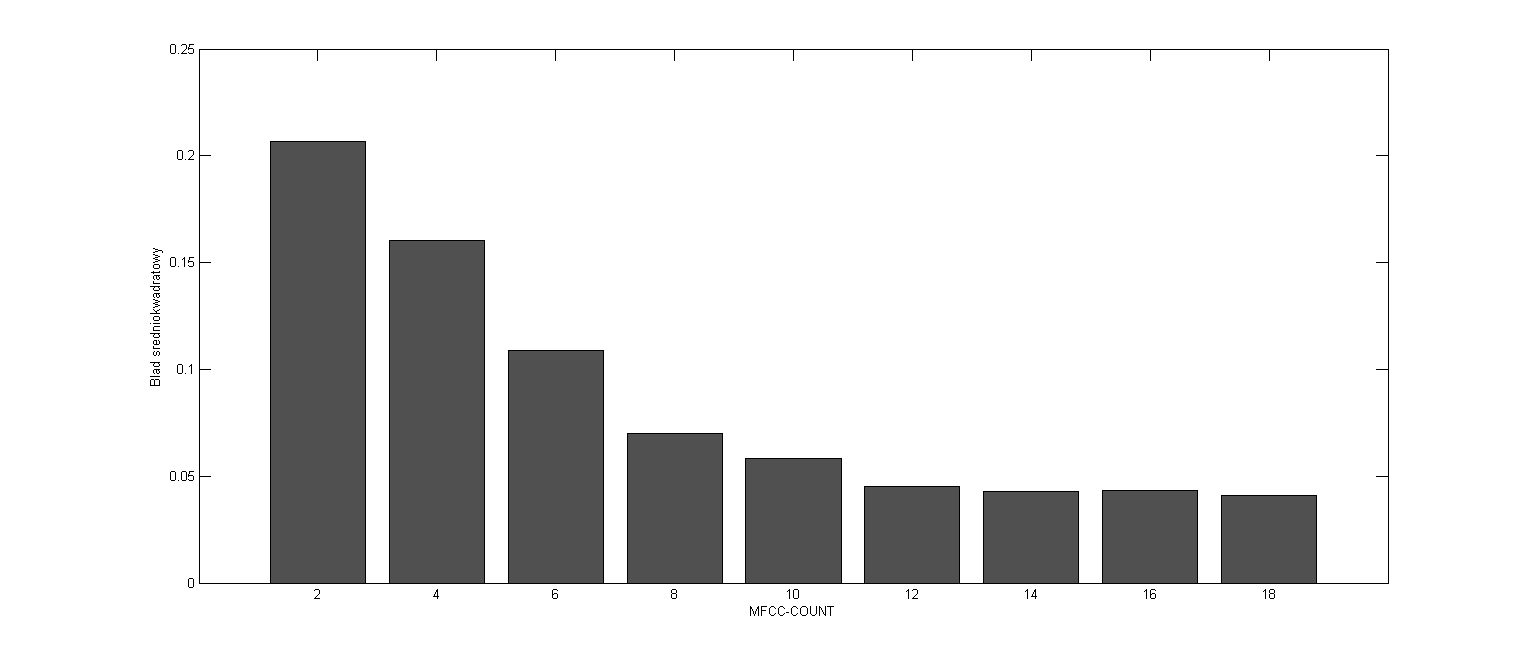
\includegraphics[width=\textwidth,trim= 3cm 0cm 3cm 0cm, clip]{./img/mfcc2}
  		\caption{Wykres prezentuje zależność błędu na zbiorze walidacyjnym od współczynnika
  		MFCC-COUNT}
  		\label{fig:mfcc2}
	\end{figure}
	Na rysunku \ref{fig:mfcc2} przedstawiono zależność błędu na zbiorze walidacyjnym od wartości 
	współczynnika FRAMES-COUNT. Z wykresu wynika że wraz z wzrostem parametru błąd ulega zmniejszeniu.
	Wydaje się że optymalna wartość tego parametru wynosi 12.
		
\section*{Bibliografia}
	\begin{itemize}
		\item
			Brian J. Love, Jennifer Vining, Xuening Sun. \textit{Automatic speaker recognition using neural networks}
		\item Lindasalwa Muda, Mumtaj Begam,I. Elamvazuthi. \textit{Voice Recognition Algorithms using Mel Frequency Cepstral Coefficient (MFCC) and Dynamic Time Warping (DTW) Techniques}
		\item
			Todor Ganchev, Nikos Fakotakis, George Kokkinakis. \textit{Comparative Evaluation of Various MFCC Implementations on the Speaker Verification Task}
		\item
			Audacity, \url{http://audacity.sourceforge.net}
		\item	
			NAudio, \url{http://naudio.codeplex.com} 
		\item
			ALGLIB, \url{http://www.alglib.net}
		\item
			Encog, \url{http://www.heatonresearch.com/encog}
	\end{itemize}
	
	\vfill
	\begin{flushright}
	$\clubsuit$ \textsc{THE END}
	\end{flushright}

\end{document}